
\section{Uniform Bundle and Item Pricing}

In this section, we show our results for uniform bundle and item pricing. Figure~\ref{fig:summary} summarizes the main results. 


\begin{figure}[t]
	\scalebox{.95}{
		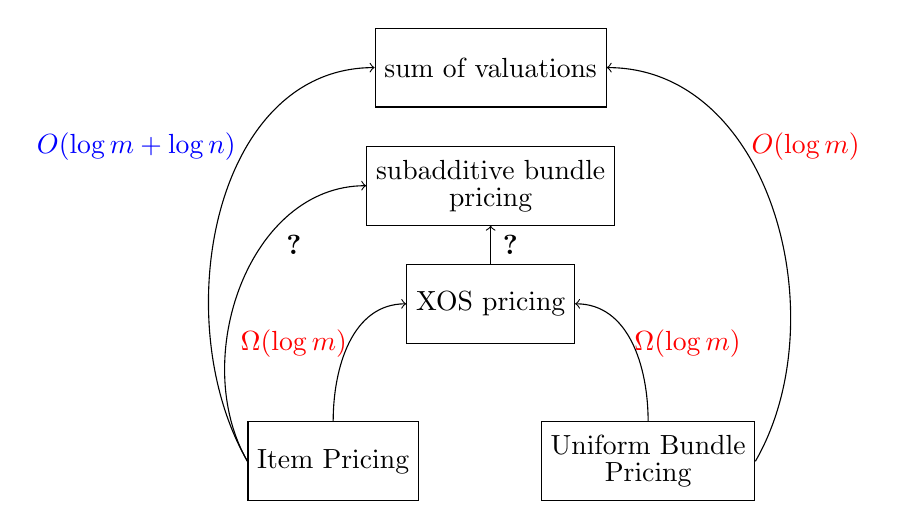
\begin{tikzpicture}
		\node (rectsum) [rectangle, draw, minimum width=7mm, minimum height=10mm] at (0,1.5) {sum of valuations};
		
		\node (rectbundle) [rectangle, draw, minimum width=7mm, minimum height=10mm] at (0,0) {\shortstack{subadditive bundle \\ pricing}};
		
		\node (rectxos) [rectangle, draw, minimum width=7mm, minimum height=10mm] at (0,-1.5) {XOS pricing};
		
		\node (rectitem) [rectangle, draw, minimum width=7mm, minimum height=10mm] at (-2,-3.5) {Item Pricing};
		
		\node (rectubundle) [rectangle, draw, minimum width=7mm, minimum height=10mm] at (2,-3.5) {\shortstack{Uniform Bundle \\ Pricing}};
		
		\draw [->] (rectubundle.east) to [out=60, in = 0] (rectsum);
		\node at (4,0.5) {\textcolor{red}{$O( \log m)$}};
		\draw [->] (rectubundle) to [out=90, in = 0] (rectxos);
		\node at (2.5,-2) {\textcolor{red}{$\Omega( \log m)$}};
		\draw [->] (rectitem.west) to [out=120, in = -180] (rectsum.west);
		\node at (-4.5,0.5) {\textcolor{blue}{$O( \log m + \log n)$}};
		\draw [->] (rectitem) to [out=90, in = -180] (rectxos.west);
		\node at (-2.5,-2) {\textcolor{red}{$\Omega( \log m)$}};
		\draw [->] (rectxos) to  (rectbundle);
		\node at (0.25,-0.75) {\textbf{?}};
		\draw [->] (rectitem.west) [out = 120, in = -180] to  (rectbundle.west);
		\node at (-2.5,-0.75) {\textbf{?}};
		
		\end{tikzpicture}
	}
	\caption{Results Summary: Red font show results in this paper; blue font shows existing known results}
	\label{fig:summary}
\end{figure}

\subsection{Uniform Bundle Pricing}

We begin by proving the $O(\log m)$ upper bound with respect to sum of valuations. 

\begin{lemma}
	Consider a hypergraph $\mH = (\mV, \mE)$ with $m$ edges and valuation $v_e$ for each edge $e \in \mE$. Then, there exists a uniform price $p'$ such that $p^{b}_e = p'$ achieves $O(\log m)$-approximation. 
\end{lemma}
\begin{proof}
	Consider the valuations $v_{e_1}, v_{e_2}, \dots, v_{e_m}$ in increasing order. We claim that $ p^{b}_e  = v_{e_{i'}}$ achieves the desired approximation for some edge $e_{i'}$. Assume for the sake of contradiction that this is not the case. Let $\textsf{OPT} = \sum_{e \in \mE} v_e$. Then $m v_{e_1} < \textsf{OPT}/ \log m$ since we can sell each edge if the bundle price is the smallest valuation. Similarly, $(m - i) v_{e_i} < \textsf{OPT}/ \log m$ for each edge. Adding up all inequalities, we get:
	
	\begin{equation}
	\begin{aligned}
	\textsf{OPT} = \sum_{e \in \mE} v_e & < \frac{\textsf{OPT}}{\log m} (\frac{1}{m} + \frac{1}{m-1} + \dots + 1) \\
	& \leq \textsf{OPT}
	\end{aligned}
	\end{equation}
	
	which is a contradiction.
\end{proof}

Next, we show that the $O(\log m)$ upper bound is tight.

\begin{lemma}
	There exists a set of buyers with XOS valuations such that any uniform bundle price produces revenue atmost $\textsf{OPT}/ \log m$.
\end{lemma}	
\begin{proof}
	Consider $n=m$ items and $m$ buyers such that buyer $b_i$ wants item $i$ for price $1/i$. It is easy to see that the valuations are XOS and achieves a revenue of $\log m$. Consider any fixed $p^b_e = 1/c$ such that $1 \leq c \leq m$. Then, the seller can sell edges that have valuation atleast $1/c$. Observe that the number of such edges is atmost $c$. Therefore, the revenue is atmost $\sum_{e:v_e \leq 1/c} 1/c = O(1)$.
\end{proof}

\subsection{Item Pricing}

Next, we show the $\Omega(\log m)$ gap between item pricing and XOS pricing.

\begin{lemma}
	There exists a set of buyers with XOS valuations such no item pricing solution can obtain revenue better than $\textsf{OPT}/ \log m$.
\end{lemma}
\begin{proof}
	Let $\mC_i$ denote the class of customers that desire exactly $\vert i \vert$ items. We construct the hypergraph instance as follows: Each class of customers $\mC_i$ has exactly $\lceil n/i \rceil$ and each customer in $\mC_i$ is assigned a partition of $i$ items such that no two customers share any item. Thus, the total number of hyperedges is $m = \sum_{i} \vert \mC_i \vert = \Theta( n \log n)$. Figure shows  an instance for $n=6$. We fix the valuation $v_e = 1$ for all hyperedges. This set of valuations is XOS and the revenue obtained by selling each edge at price $p^{b}_e = 1$ extracts the full revenue of $\Theta(n \log n)$.
	
	Next, we show that no item pricing solution can do better than $O(n)$. We will show this by induction on the customer class $\mC_i$. The base case is revenue obtained by selling edges to customers in $\mC_1$. Since there are atmost $n$ edges, the maximum revenue is $O(n)$. Consider the customer class $\mC_k$. Let denote $0 < \alpha \leq 1$ be the fraction of edges sold to customers in $\mC_k$ and let $\mE_k$ denote such edges. Then, the maximum revenue that can be extracted is $\alpha \lceil n/k \rceil$. We distinguish three types of edges: $(i)$ edges that share atleast one item with edges in $\mE_k$ $(ii)$ edges that do not share any item with edges in $\mE_k$ $(iii)$ edges that are strictly contained within $\mE_k$. By the induction hypothesis, the maximum revenue that can be extracted from all type $(ii)$ edges is atmost $O(n)$. Each edge in $\mE_k$ can overlap with atmost $2(k-1)$ edges that have size strictly lesser than $k$. Thus, the revenue extracted from type $(i)$ edges is atmost $2(k-1) \alpha \lceil n/k \rceil = O(n)$. Consider an edge $e' \in \mE_k$ and let $w_1, \dots w_k$ be the weights of items in $e'$. Since the seller is able to sell $e'$, we have that $w_1 + \dots w_k \leq 1$. Observe that the maximum revenue of all edges of size strictly lesser than $k$ (say $k'$) using items in $e'$ is also atmost $w_1 + \dots w_k \leq 1$ which gives revenue of $O(k)$. 
\end{proof}

